\section{Selection Results}

Before addressing the research questions, a descriptive characterization of the 19 selected articles is presented. This analysis contextualizes the state of the field by examining the temporal evolution of publications, geographic concentration, methodological diversity, and sectoral coverage of the included studies.

% ── 1. TEMPORAL ─────────────────────────────────────────────────────────────
\subsection{Temporal Distribution}

\begin{figure}[h]
\centering
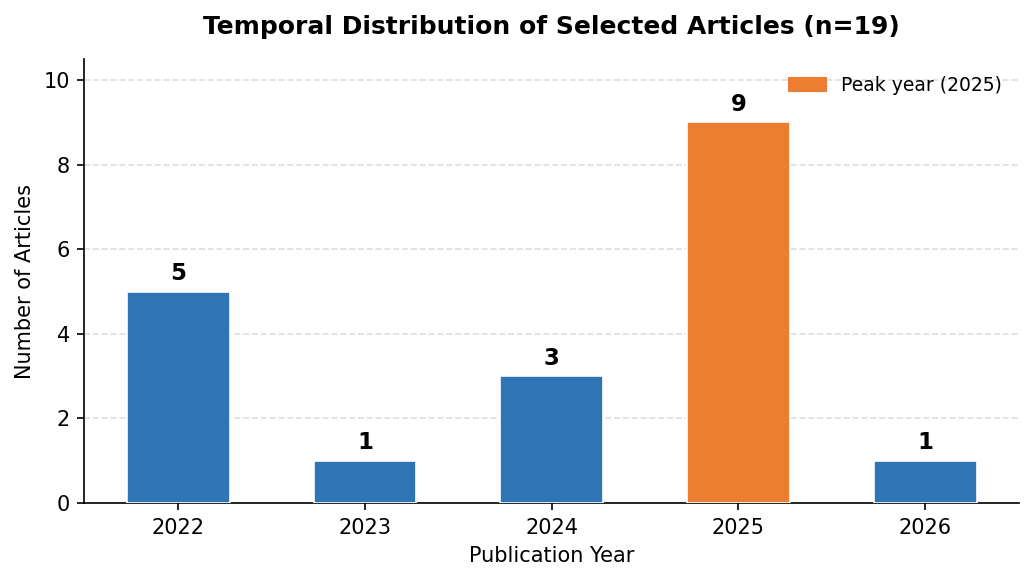
\includegraphics[width=0.75\textwidth]{figures/temporal.png}
\caption{Temporal distribution of selected articles (n=19).}
\label{fig:temporal}
\end{figure}

The temporal distribution of the 19 selected articles (Fig.~\ref{fig:temporal}) reveals a clear acceleration in research activity at the intersection of Artificial Intelligence and Supply Chain Risk Management (SCRM) over recent years. The earliest cluster (2022) accounts for five publications, coinciding with a period of heightened academic interest driven by the operational disruptions caused by the COVID-19 pandemic and subsequent supply chain instability. A relative consolidation is observed in 2023 (n=1) and 2024 (n=3), suggesting a transitional period as the field matured and pivoted towards more technically sophisticated approaches.

The most notable finding is the sharp surge in 2025, which alone concentrates nine of the nineteen articles (47.4\%), representing the single most productive year in the corpus. This trajectory strongly indicates that the application of AI to SCRM is an emergent and rapidly evolving domain, where foundational conceptual work (2022) is giving way to empirical validation and system deployment (2025–2026). The presence of one article from 2026 further corroborates that the research frontier is active and ongoing, underscoring the timeliness and relevance of this systematic review.

% ── 2. GEOGRAPHY ─────────────────────────────────────────────────────────────
\subsection{Geographic Distribution}

\begin{figure}[h]
\centering
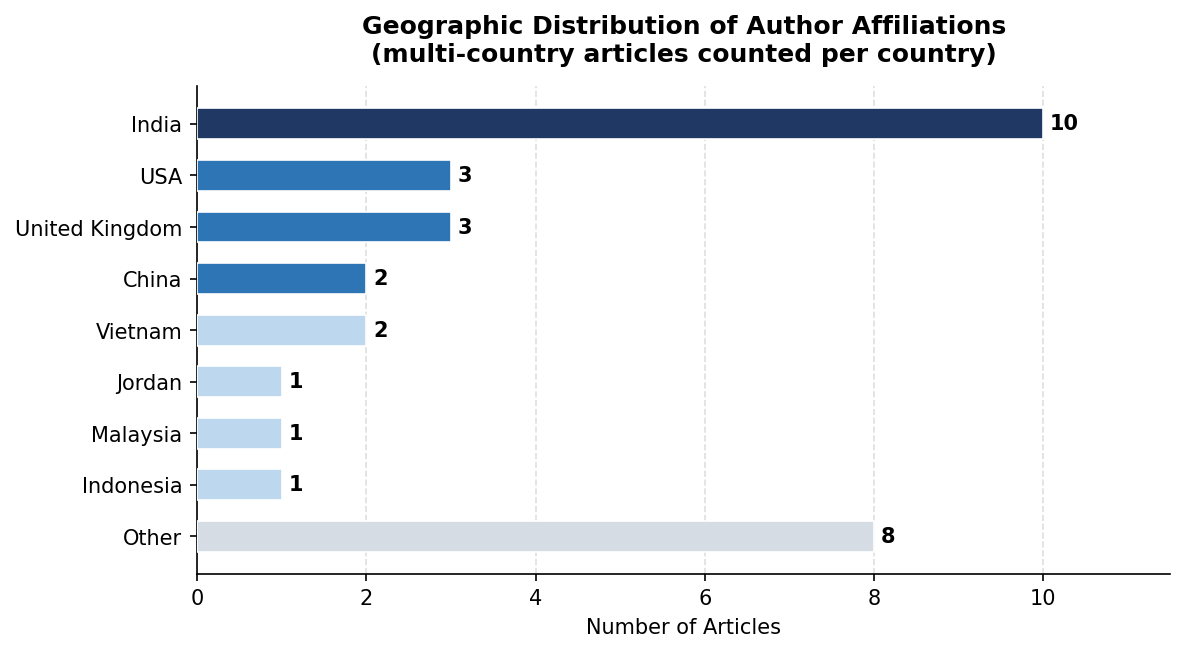
\includegraphics[width=0.85\textwidth]{figures/geography.png}
\caption{Geographic distribution of author affiliations (multi-country articles counted per country, n=19).}
\label{fig:geography}
\end{figure}

The geographic analysis (Fig.~\ref{fig:geography}) reveals a pronounced concentration of research output originating from Asia and Anglo-Saxon academic contexts. India emerges as the dominant contributor, with affiliations appearing in ten of the nineteen articles, a figure that reflects both the country's substantial investment in AI research capacity and the strategic importance of supply chain resilience in its manufacturing and logistics sectors. The United States (n=3) and United Kingdom (n=3) follow, consistent with their historically strong publication output in operations management and computer science. China (n=2) and Vietnam (n=2) are also represented, both nations with significant stakes in global manufacturing networks.

A critical observation is the near-complete absence of European and South American authorship. With the exception of one article from Germany and one from Hungary (both as co-authors in multi-country collaborations), the European research community appears largely underrepresented in this specific intersection of AI and SCRM. This constitutes a meaningful geographic gap, as European supply chains—heavily regulated and deeply integrated through European Union frameworks—may face distinct risk profiles not adequately captured by models developed in other geopolitical and industrial contexts. Future research should prioritize geographically diverse empirical studies to ensure generalizability.

% ── 3. STUDY TYPE ─────────────────────────────────────────────────────────────
\subsection{Study Type and Methodological Profile}

\begin{figure}[H]
\centering
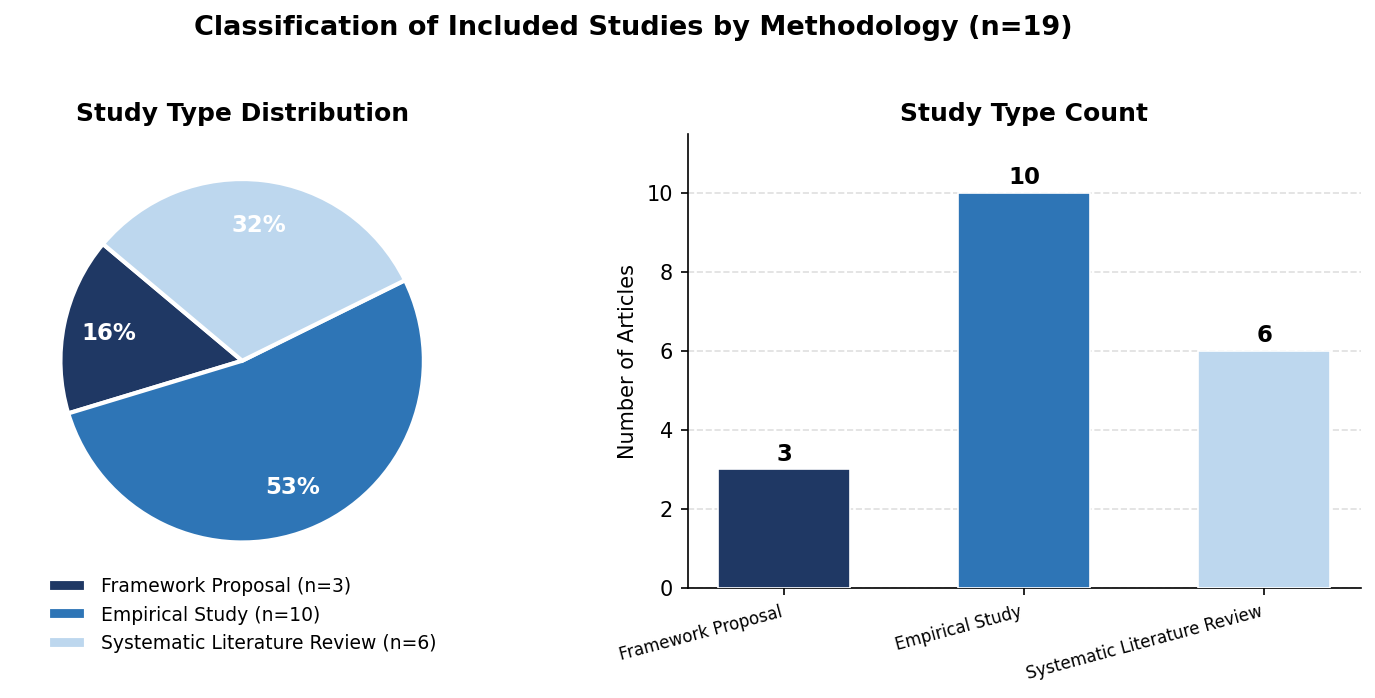
\includegraphics[width=\textwidth]{figures/study_type.png}
\caption{Classification of included studies by methodology (n=19).}
\label{fig:studytype}
\end{figure}

The methodological profile of the corpus (Fig.~\ref{fig:studytype}) is dominated by \textit{Empirical Studies} (n=10, 52.6\%), which encompass case studies, computational experiments with real or simulated datasets, and validation studies applying AI models to supply chain data. This predominance signals that the field has progressed beyond purely theoretical discussion and is actively engaged in operationalizing AI solutions in applied settings.

\textit{Systematic Literature Reviews} (SLR) constitute the second largest group (n=6, 31.6\%), including bibliometric analyses and state-of-the-art reviews. The presence of six SLRs within a 19-article corpus is noteworthy, as it suggests that the community itself recognizes the need for synthesis and consolidation—a signal that the field is reaching a level of maturity where meta-analytical work is valued alongside primary research. This also implies that the knowledge base, while growing rapidly, remains fragmented, warranting ongoing integrative efforts such as the present review.

\textit{Framework Proposals} (n=3, 15.8\%) round out the corpus, representing conceptual contributions that map AI architectures and processes for SCRM without full empirical validation. These works serve as design blueprints for future implementations but highlight a gap: further empirical testing of proposed frameworks in real-world, longitudinal supply chain settings remains scarce.

% ── 4. SECTORS ─────────────────────────────────────────────────────────────
\subsection{Sectoral Coverage}

\begin{figure}[H]
\centering
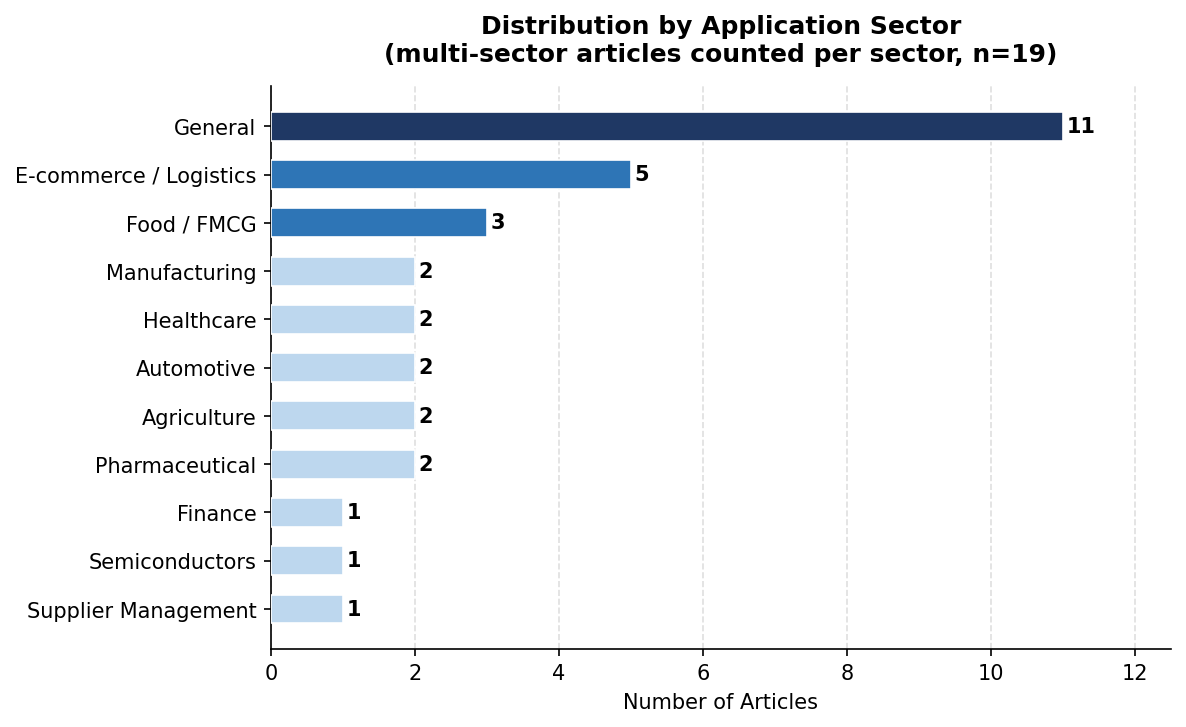
\includegraphics[width=0.85\textwidth]{figures/sectors.png}
\caption{Distribution of articles by application sector (multi-sector articles counted per sector, n=19).}
\label{fig:sectors}
\end{figure}

The sectoral analysis (Fig.~\ref{fig:sectors}) exposes a significant limitation in the current literature: the majority of articles (n=11) adopt a \textit{general} scope, applying AI-based SCRM frameworks without targeting a specific industry vertical. While such generality offers broad applicability, it simultaneously limits practical guidance for practitioners operating within sectors subject to idiosyncratic regulatory, operational, and risk environments.

Among sector-specific contributions, \textit{E-commerce and Logistics} (n=5) represents the most investigated context, reflecting the real-time data availability and transaction volume that make this sector particularly well-suited to AI-driven risk detection. \textit{Food and FMCG}, \textit{Healthcare}, \textit{Automotive}, \textit{Agriculture}, and \textit{Pharmaceuticals} each appear in two articles, indicating nascent but emerging interest. Notably, sectors such as \textit{Financial Services}, \textit{Semiconductors}, and \textit{Energy}—all of which face severe and well-documented supply chain vulnerabilities—are critically underrepresented.

This sectoral breadth gap is a substantive finding of this review. It implies that the AI techniques currently proposed may not be calibrated to sector-specific risk taxonomies, compliance constraints, or data infrastructures, and that domain-adapted AI models represent a priority avenue for future research.

% ── 5. AI TECHNIQUES ─────────────────────────────────────────────────────────
\subsection{Frequency of AI Techniques}

\begin{figure}[h]
\centering
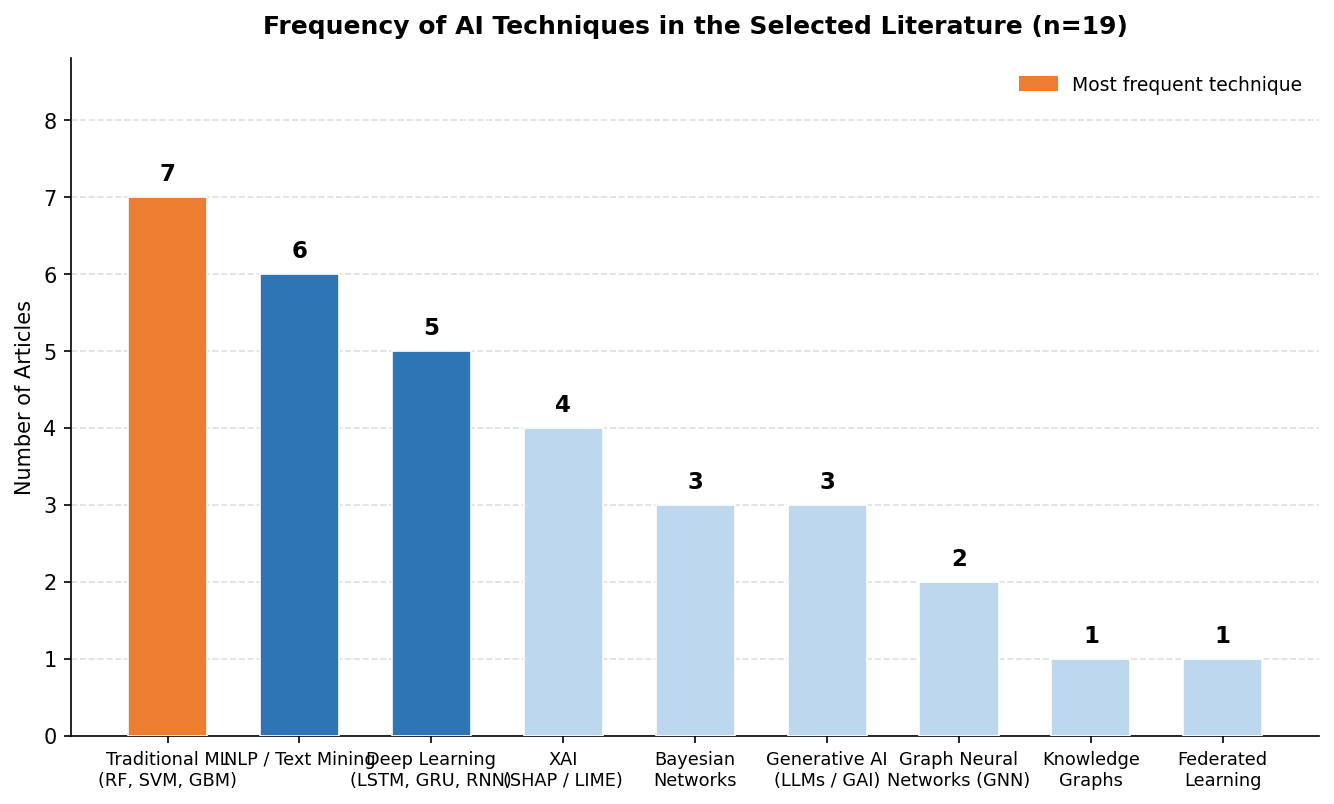
\includegraphics[width=\textwidth]{figures/techniques.png}
\caption{Frequency of AI techniques identified across the selected literature (n=19).}
\label{fig:techniques}
\end{figure}

The frequency analysis of AI techniques employed across the corpus (Fig.~\ref{fig:techniques}) reveals a clear hierarchy in adoption, with established, interpretable methods predominating over state-of-the-art generative or graph-based approaches.

\textit{Traditional Machine Learning} (RF, SVM, GBM, and variants) is the most prevalent technique, appearing in seven articles. Its dominance is attributable to its strong performance on structured tabular data—the dominant format in ERP, WMS, and supplier management systems—as well as its relative computational efficiency and interpretability compared to deeper architectures. \textit{NLP and Text Mining} (n=6) constitutes the second most frequent category, reflecting the growing recognition that unstructured data sources—social media, news feeds, regulatory announcements—contain early signals of supply chain stress that structured internal data cannot capture.

\textit{Deep Learning} architectures (LSTM, GRU, RNN; n=5) rank third, used primarily for sequential and time-series forecasting tasks. \textit{Explainable AI} (SHAP, LIME; n=4) has gained meaningful traction, consistent with a growing demand for algorithmic transparency in high-stakes operational contexts. \textit{Bayesian Networks} (n=3) and \textit{Generative AI} (LLMs, GAI; n=3) appear with equal frequency, although their use cases differ markedly: the former for probabilistic multi-factor risk assessment, the latter for processing unstructured disruption signals.

At the lower end of adoption, \textit{Graph Neural Networks} (n=2), \textit{Knowledge Graphs} (n=1), and \textit{Federated Learning} (n=1) remain niche despite their theoretical promise for modelling interconnected supply network topologies and privacy-preserving collaborative risk management, respectively. This underrepresentation is a pivotal finding: techniques most suited to the networked, relational nature of supply chains are the least deployed, suggesting that the field has not yet fully leveraged the structural characteristics of its own domain.